\section{Semantics and System Model}
\label{sec:ra-def}

In this section, we formalize Read Atomic isolation and, to capture
scalability, formulate a pair of strict scalability criteria:
coordination-free execution and partition independence. Readers more interested in
RAMP algorithms may wish to proceed to Section~\ref{sec:ramp-algorithm}.

\subsection{RA Isolation: Formal Specification}
\label{sec:ra-spec}

To formalize RA isolation, as is standard~\cite{adya,bernstein-book} (and as in
Chapter~\ref{c.isolation}), we consider
ordered sequences of reads and writes to arbitrary sets of items, or
transactions. We call the set of items a transaction reads from and
writes to its \textit{item read set} and \textit{item write set}. Each
write creates a \textit{version} of an item and we identify versions
of items by a \textit{timestamp} taken from a totally ordered set
(e.g., natural numbers) that is unique across all versions of each
item. Timestamps therefore induce a total order on versions of each
item, and we denote version $i$ of item $x$ as $x_i$. All items have
an initial version $\bot$ that is located at the start of each order
of versions for each item and is produced by an initial transaction
$T_\bot$. Each transaction ends in a \textit{commit} or an
\textit{abort} operation; we call a transaction that commits a
\textit{committed} transaction and a transaction that aborts a
\textit{aborted} transaction. In our model, we consider
\textit{histories} comprised of a set of transactions along with their
read and write operations, versions read and written, and commit or
abort operations. In our example histories, all transactions commit
unless otherwise noted.

\begin{definition}[Fractured Reads]
  A transaction $T_j$ exhibits the \textit{fractured reads} phenomenon
  if transaction $T_i$ writes versions $x_a$ and $y_b$ (in any order,
  where $x$ and $y$ may or may not be distinct items), $T_j$ reads
  version $x_a$ and version $y_c$, and $c < b$.
\end{definition}

We also define Read Atomic isolation to prevent transactions from
reading uncommitted or aborted writes. This is needed to capture the
notion that, under RA isolation, readers only observe the final output
of a given transaction that has been accepted by the database. To do
so, we draw on existing definitions from the literature on weak
isolation.

Our RAMP protocols provide this property by assigning the final write
to each item in each transaction the same timestamp. However, to avoid
further confusion between the standard practice of assigning each
final write in a serializable multi-version history the same
timestamp~\cite{bernstein-book} and the flexibility of timestamp
assignment admitted in Adya's formulation of weak isolation, we
continue with the above definitions.

These criteria prevent readers from observing \textit{uncommitted}
versions (i.e., those produced by a transaction that has not committed
or aborted), \textit{aborted} versions (i.e., those produced by a
transaction that has aborted), or \textit{intermediate} versions
(i.e., those produced by a transaction but were later overwritten by
writes to the same items by the same transaction).

We can finally define Read Atomic isolation:

\begin{definition}[Read Atomic]
  A system provides \textit{Read Atomic} isolation (RA) if it prevents
  fractured reads phenomena and also prevents transactions from
  reading uncommitted, aborted, or intermediate versions (i.e., Adya's
  \textit{G0}, \textit{G1a}, \textit{G1b}, \textit{G1c}).
\end{definition}

Thus, RA informally provides transactions with a ``snapshot'' view of
the database that respects transaction boundaries (see
Sections~\ref{sec:ra-compare} and~\ref{sec:ra-serializable} for more
details, including a discussion of transitivity). RA is simply a
restriction on read \textit{visibility}---if the ACID ``Atomicity''
property requires that all or none of a transaction's updates are
performed, RA requires that all or none of a transaction's updates are
visible to other transactions.

Importantly, RA is \iconfluent: if two read/write histories each
independently do not have fractured reads, composing them will not
change the values returned by any read operations. This means that
there is at least one coordination-free implementation of RA, which we will
develop in Section~\ref{sec:ramp-algorithm}.

\subsection{RA Implications and Limitations}
\label{sec:usage}

As outlined in Section~\ref{sec:usecases}, RA isolation matches
several common use cases. However, RA is \textit{not} sufficient for
all applications. RA does not prevent concurrent updates or provide
serial access to data items; that is, under RA, two transactions are
never prevented from both producing different versions of the same
data items. For example, RA is an incorrect choice for an application
that wishes to maintain positive bank account balances in the event of
withdrawals. RA is a better fit for our ``friend'' operation because
the operation is write-only and correct execution (i.e., inserting
both records) is not conditional on concurrent updates.

From a programmer's perspective, we have found RA isolation to be most
easily understandable (at least initially) with read-only and
write-only transactions; after all, because RA allows concurrent
writes, any values that are read might be changed at any
time. However, read-write transactions are indeed well defined under
RA.

To handle conflicting operations, RA isolation benefits from the use
of commutative and associative merge functions. The default behavior
we present here is a ``last write wins'' policy, with ties broken
according to version. However, more sophisticated datatypes such as
commutative replicated sets, counters, and maps~\cite{crdt} are also
useful, especially for data structures such as index entries.

To illustrate these points, in Section~\ref{sec:ra-compare}, we
describe RA's relation to other formally defined isolation levels,
and, in Section~\ref{sec:ra-serializable}, we discuss when RA provides
serializable outcomes.

\subsection{RA Compared to Other Isolation Models}
\label{sec:ra-compare}

In this section, we illustrate RA's relationship to alternative weak
isolation models by both example and reference to particular isolation
phenomena drawn from~\cite{adya} and~\cite{hat-vldb}. Formal
definitions of the models below can be found in in
Section~\ref{sec:hat-definitions}

RA is stronger than Read Committed as Read Committed does not prevent
fractured reads. History~\ref{hist:rc} does not respect RA
isolation. After $T_1$ commits, both $T_2$ and $T_3$ could both commit
but, to prevent fractured reads, $T_4$ and $T_5$ must
abort. History~\ref{hist:rc} respects RC isolation and all
transactions can safely commit.

\begin{eqnarray}
\label{hist:rc}
T_1 & w(x_1); w(y_1)\\
T_2 & r(x_\bot); r(y_\bot)\nonumber\\
T_3 & r(x_1); r(y_1)\nonumber\\
T_4 & r(x_\bot); r(y_1)\nonumber\\
T_5 & r(x_1); r(y_\bot)\nonumber 
\end{eqnarray}

\minihead{Lost Updates} Lost Updates phenomena informally occur when two
transactions simultaneously attempt to make conditional modifications to
the same data item(s).

RA does not prevent Lost Updates phenomena. History~\ref{hist:lostupdate}
exhibits the Lost Updates phenomenon but is valid under RA. That is,
$T_1$ and $T_2$ can both commit under RA isolation.

\begin{eqnarray}
\label{hist:lostupdate}
T_1 & r(x_\bot); w(x_1)\\
T_2 & r(x_\bot); w(x_2)\nonumber
\end{eqnarray}

History~\ref{hist:lostupdate} is invalid under a stronger isolation
model that prevents Lost Updates phenomena, such as Snapshot Isolation
or Cursor Isolation. Under either of these models, the system would
abort $T_1$, $T_2$, or both. However, Cursor Stability does not
prevent fractured reads phenomena, so RA and Cursor Stability are
incomparable.

\minihead{Write Skew} RA does not prevent Write Skew
phenomena. History~\ref{hist:writeskew} exhibits the Write Skew
phenomenon (Adya's $G2$) but is valid under RA. That is, $T_1$ and
$T_2$ can both commit under RA isolation.

\begin{eqnarray}
\label{hist:writeskew}
T_1 & r(y_\bot); w(x_1)\\
T_2 & r(x_\bot); w(y_2)\nonumber
\end{eqnarray}

History~\ref{hist:writeskew} is invalid under a stronger isolation
model that prevents Write Skew phenomena. One stronger model is
Repeatable Read. Under Repeatable Read isolation, the system would
abort either $T_1$, $T_2$, or both. (Importantly, Adya's formulation
of Repeatable Read is considerably stronger than the ANSI SQL standard
specification; RA is stronger than the Cut Isolation we consider in
Chapter~\ref{c.isolation}.)


\minihead{Missing dependencies} Notably, RA does not---on its
own---prevent missing dependencies---in effect, missing transitive
updates. We again reproduce Adya's definitions below:

\begin{definition}[Missing Transaction Updates]
A transaction $T_j$ misses the effects of a transaction $T_i$ if $T_i$
writes $x_i$ and commits and another transaction $T_j$ reads another
version $x_k$ such that $k < i$; i.e., $T_j$ reads a version of $x$
that is older than the version that was committed by $T_i$.
\end{definition}

Adya subsequently defines a criteria that prohibits missing
transaction updates across all types of dependency edges:

\begin{definition}[No-Depend-Misses]
If transaction $T_j$ depends on transaction $T_i$, $T_j$ does not miss
the effects of $T_i$.
\end{definition}

History~\ref{hist:missingdeps} does not exhibit the No-Depend-Misses
phenomenon but is still valid under RA. That is, $T_1$, $T_2$, and
$T_3$ can all commit under RA isolation. Thus, fractured reads
prevention is similar to No-Depend-Misses but only applies to
immediate read dependencies (rather than all transitive dependencies).

\begin{eqnarray}
\label{hist:missingdeps}
T_1 & w(x_1); w(y_1)\\
T_2 & r(y_1); w(z_2)\nonumber\\
T_3 & r(x_\bot); r(z_2) \nonumber
\end{eqnarray}

History~\ref{hist:missingdeps} is invalid under a stronger isolation
model that prevents missing dependencies phenomena, such as standard
semantics for Snapshot Isolation (notably, not Parallel Snapshot
Isolation~\cite{walter}) and Repeatable Read isolation. Under one of
these models, the system would abort either $T_3$ or all of $T_1$,
$T_2$, and $T_3$.

This behavior is particularly important to the use cases that we
discuss in Sections~\ref{sec:usage} and~\ref{sec:ra-serializable}:
writes that should be read together should be written together.

We further discuss the benefits and enforcements of transitivity in
Section~\ref{sec:causal}.

\minihead{OTV and Many-Preceders} As noted in
Section~\ref{sec:rampr}, the Fractured Reads phenomenon subsumes
the Observed Transaction Vanishes and Many-Preceders phenomena from
Chapter~\ref{c.isolation}. To illustrate:

If $T_j$ exhibits the OTV phenomenon reads $x_a$ produced by $T_i$ in
the definition of Fractured Reads above then there is a
read-dependency edge by $x$ from $T_j$ to $T_i$ in $USG(H)$; however,
if $T_j$ also reads $y_c$ and $c < b$, then $T_i$ must anti-depend on
$T_j$, resulting in OTV. Thus, every fractured read is an instance of
OTV. However, not every fractured read is an instance of OTV. That is,
in our example, if $T_j$ reads $y_b$ and then reads $y_c$, fractured
reads have occurred, but OTV has not (due to the clause that ``$T_j$'s
read from $y$ precedes its read from $x$'' in
Definition~\ref{def:otv}).

Fractured reads also subsumes the many-preceders phenomenon (in the
item-specific case, Definition~\ref{def:imp}). If $T_i$ exhibits the
IMP phenomenon, it directly item-depends by $x$ on more than one
transaction---say, $T_j$ and $T_k$---then $T_i$ read versions $x_i$
and $x_k$ produced by each of $T_i$ and $T_k$. However, by definition,
$i < k$ or $k < i$, and thus $T_j$ also has fractured reads. Again,
not every fractured read is an instance of IMP. Consider the following
history:
\begin{eqnarray}
T_1 & w(x_1); w(y_1)\\
T_2 & r(x_\bot); r(y_1)\nonumber
\end{eqnarray}
$T_2$ exhibits fractured reads but does not exhibit IMP.

\minihead{Predicates} Thus far, we have not extensively discussed the
use of predicate-based reads. As Adya notes~\cite{adya} and
we describe above, predicate-based isolation guarantees can be cast as
an extension of item-based isolation guarantees (see also Adya's
\textit{PL-2L}, which closely resembles RA). RA isolation is no
exception to this rule. We can extend each RA definition to include
predicates using Adya's predicate-based formalism.

\minihead{Relating to Additional Guarantees} RA isolation subsumes
several other useful guarantees. RA prohibits Item-Many-Preceders and Observed
Transaction Vanishes phenomena; RA also guarantees Item Cut
Isolation, and with predicate support, RA subsumes
Predicate Cut Isolation Thus, it is a combination of
Monotonic Atomic View and Item Cut Isolation (Section~\ref{sec:anomalies-hat}).
\minihead{Summary} Figure~\ref{fig:isolation} relates RA isolation to
several existing models. RA is stronger than Read Committed, Monotonic
Atomic View, and Cut Isolation, weaker than Snapshot
Isolation, Repeatable Read, and Serializability, and incomparable to
Cursor Stability.


\begin{figure}
\begin{center}
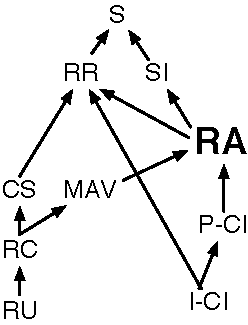
\includegraphics[width=1.3in]{diagram/isolation-graffle.pdf}
\end{center}
\caption{Comparison of RA with isolation levels
  from~\cite{adya,hat-vldb}. RU: Read Uncommitted, RC: Read
  Committed, CS: Cursor Stability, MAV: Monotonic Atomic View, ICI:
  Item Cut Isolation, PCI: Predicate Cut Isolation, RA: Read Atomic,
  SI: Snapshot Isolation, RR: Repeatable Read (Adya \textit{PL-2.99}), S:
  Serializable.}
\label{fig:isolation}
\end{figure}

\subsection{RA and Serializability}
\label{sec:ra-serializable}

When we began this work, we started by examining the use cases
outlined in Section~\ref{sec:motivation} and deriving a weak isolation
guarantee that would be sufficient to ensure their correct
execution. For general-purpose read-write transactions, RA isolation
may indeed lead to non-serializable (and possibly incorrect) database
states and transaction outcomes. Yet, as Section~\ref{sec:usage}
hints, there appears to be a broader ``natural'' pattern for which RA
isolation appears to provide an intuitive (even ``correct'')
semantics. In this section, we show that for transactions
with a particular property of their item read and item write sets, RA is, in
fact, serializable. We define this property, called the
\textit{read-subset-items-written (RSIW) property}, prove that transactions
obeying the RSIW property lead to serializable outcomes, and discuss
the implications of the RSIW property for the applications outlined in
Section~\ref{sec:motivation}.

Because our system model operates on multiple versions, we must make a
small refinement to our use of the term ``serializability''---namely,
we draw a distinction between serial and one-copy serializable
schedules, per Bernstein et al.~\cite{bernstein-book}. First, we say that two histories
$H_1$ and $H_2$ are \textit{view equivalent} if they contain the same
set of committed transactions and have the same operations and $DSG(H_1)$
and $DSG(H_2)$ have the same direct read dependencies. For
consistency with prior work, we say that $T_i$ \textit{reads from}
$T_j$ if $T_i$ directly read-depends on $T_j$. We say that a
transaction is \textit{read-only} if it does not contain write
operations and that a transaction is \textit{write-only} if it does
not contain read operations. In this section, we concern ourselves
with \textit{one-copy serializability}~\cite{bernstein-book}, which we
define using the previous definition of view equivalence.

\begin{definition}[One-Copy Serializability]
  A history is one-copy serializable if it is view equivalent to a serial
  execution of the transactions over a single logical copy of the
  database.
\end{definition}

The basic intuition behind the RSIW property is straightforward: under
RA isolation, if application developers use a transaction to bundle a
set of writes that should be observed together, any transactions that
read from the items that were written will, in fact, behave ``properly''---or
one-copy serializably. That is, for read-only and write-only transactions, if
each reading transaction only reads a subset of the items that another
write-only transaction wrote, then RA isolation is equivalent to
one-copy serializable isolation. Before proving that this behavior is
one-copy serializable, we can more precisely characterize this condition as
follows:

\begin{definition}[Read-Subset-Items-Written] A read-only transaction
  $T_r$ exhibits the \textit{Read-Subset-Items-Written} property if,
  whenever $T_r$ reads a version produced by a write-only transaction
  $T_w$, $T_r$ only reads items written to by $T_w$.
\end{definition}

For example, consider the following History~\ref{hist:rsw}:
\begin{eqnarray}
\label{hist:rsw}
T_1 & w(x_1); w(y_1)\\
T_2 & r(x_1); w(y_1)\nonumber\\
T_3 & r(x_1); r(z_\bot)\nonumber
\end{eqnarray}

Under History~\ref{hist:rsw}, $T_2$ exhibits the RSIW property because
it reads a version produced by transaction $T_1$ and its item read set
($\{x,y\}$) is a subset of $T_1$'s item write set ($\{x,y\}$). However,
$T_3$ does not exhibit the RSIW property because $i.)$ $T_3$ reads from
$T_1$ but $T_3$'s read set ($\{x,z\}$) is not a subset of $T_1$'s
write set ($\{x,y\}$) and $ii.)$, perhaps more subtly, $T_3$ reads
from both $T_1$ and $T_\bot$.

We say that a history $H$ containing read-only and write-only
transactions exhibits the RSIW property (or \textit{has RSIW}) if every read-only transaction
in $H$ exhibits the RSIW property.

This brings us to our main result in this section:

\begin{theorem}
\label{thm:rsw}
If a history $H$ containing read-only and write-only transactions
has RSIW and is valid under RA isolation, then
$H$ is one-copy serializable.
\end{theorem}

The proof of Theorem~\ref{thm:rsw} is by construction: given a history
$H$ has RSIW and is valid under RA isolation, we
describe how to derive an equivalent one-copy serial execution of the
transactions in $H$. We begin with the construction procedure, provide examples
of how to apply the procedure, then prove that the procedure
converts RSIW histories to their one-copy serial equivalents. We
provide the proof in Section~\ref{sec:rsiwproof}

\minihead{Utility} Theorem~\ref{thm:rsw} is helpful because it
provides a simple syntactic condition for understanding when RA will
provide one-copy serializable access. For example, we can apply this
theorem to our use cases from Section~\ref{sec:motivation}. In the
case of multi-entity update and read, if clients issue read-only and
write-only transactions that obey the RSIW property, their result sets
will be one-copy serializable. The RSIW property holds for
equality-based lookup of single records from an index (e.g., fetch
from the index and subsequently fetch the corresponding base tuple,
each of which was written in the same transaction (e.g., was
auto-generated upon insertion of the tuple into the base
relation). However, the RSIW property does not in the event of
multi-tuple reads, leading to less intuitive behavior. Specifically,
if two different clients trigger two separate updates to an index
entry, some clients may observe one update but not the other, and
other clients may observe the opposite behavior. In this case, the
RAMP protocols still provide a snapshot view of the database according
to the index(es)---that is, clients will never observe base data that
is inconsistent with the index entries---but nevertheless surface
non-serializable database states. Finally, for more general
materialized view accesses, point queries and bulk insertions have
RSIW.

As discussed in Section~\ref{sec:motivation}, in the case of indexes
and views, it is helpful to view each physical data structure (e.g.,
a CRDT~\cite{crdt} used to represent an index entry) as a
\textit{collection} of versions. In this case, the RSIW property
applies only if clients make modifications to the entire collection at
once (e.g., as in a \texttt{DELETE CASCADE} operation).

Coupled with an appropriate algorithm ensuring RA isolation, we can
ensure one-copy serializable isolation. This addresses a long-standing
concern with our work: why is RA somehow ``natural'' for these use
cases (but not necessarily all use cases)?  We have encountered
applications that do not require one-copy serializable access---such
as the mailbox unread message maintenance from
Section~\ref{sec:motivation} and, in some cases, index maintenance for
non-read-modify-write workloads---and therefore may safely violate
RSIW. However, we believe the RSIW property is a handy principle (or,
at the least, rule of thumb) for reasoning about applications of RA
isolation and the RAMP protocols.

Finally, the RSIW property is only a \textit{sufficient} condition for
one-copy serializable behavior under RA isolation. It is not
necessary---for example, there are several alternative sufficient
conditions to consider. As a natural extension, while RSIW only
pertains to pairs of read-only and write-only transactions, one might
consider allowing readers to observe multiple write transactions. For
example, consider the following history:
\begin{eqnarray}
\label{hist:rsw-multi-right}
T_1 & w(x_1); w(y_1)\\
T_2 & w(u_2); w(z_2)\nonumber\\
T_3 & r(x_1); r(z_2)\nonumber
\end{eqnarray}
History~\ref{hist:rsw-multi-right} is valid under RA and is also
one-copy serializable but does not have RSIW: $T_3$ reads from
\textit{two} transactions' write sets. However, consider the following
history:
\begin{eqnarray}
\label{hist:rsw-multi-wrong}
T_1: & w(x_1); w(y_1)\\
T_2: & w(u_2); w(z_2)\nonumber\\
T_3: & r(x_1); r(z_\bot)\nonumber\\
T_4: & r(x_\bot); r(z_2)\nonumber
\end{eqnarray}
History~\ref{hist:rsw-multi-wrong} is valid under RA, consists only of
read-only and write-only transactions, yet is no longer
one-copy serializable. $T_3$ observes, in effect, a one-copy serializable prefix
beginning with $T_\bot; T_1$ while $T_4$ observes a prefix beginning
with $T_\bot; T_2$. Neither $T_3$ nor $T_4$ observes the prefixes
$T_\bot; T_1; T_2$ or $T_\bot; T_2; T_1$.

Thus, while there may indeed be useful criteria beyond the RSIW
property that we might consider as a basis for one-copy serializable
execution under RA, we have observed RSIW to be the most intuitive and
useful thus far. One clear criteria is to search for schedules or
restrictions under RA with an acyclic Directed Serialization Graph (from
Appendix~\ref{sec:rsiwproof}). The reason why RSIW is so simple for
read-only and write-only transactions is that each read-only
transaction only reads from one other transaction and does not induce
any additional anti-dependencies. Combining reads and writes
complicates reasoning about the acyclicity of the graph.

This exercise touches upon an important
lesson in the design and use of weakly isolated systems: by
restricting the set of operations accessible to a user (e.g., RSIW
read-only and write-only transactions), one can often achieve more
scalable implementations (e.g., using weaker semantics)
\textit{without} necessarily violating existing abstractions (e.g.,
one-copy serializable isolation). While prior work often focuses on
restricting only operations (e.g., to read-only or write-only
transactions~\cite{eiger,divy-writeonly}, or stored
procedures~\cite{calvin,hstore,jones-dtxn}, or single-site
transactions~\cite{megastore}) or only semantics (e.g., weak isolation
guarantees~\cite{hat-vldb,eiger,explicit-socc}), we see
considerable promise in better understanding the intersection between
and combinations of the two. This is often subtle and almost always
challenging, but the results---as we found here---may be surprising.

 \subsection{System Model and Scalability}
\label{sec:sysmodel}

We consider databases that are partitioned, with the set of items in
the database spread over multiple servers. Each item has a single
logical copy, stored on a server---called the item's
\textit{partition}---whose identity can be calculated using the
item. Clients forward operations on each item to the item's partition,
where they are executed. In our examples, all data items have the null
value ($\bot$) at database initialization. In this section, we do not
model replication of data items within a partition; this can happen at
a lower level of the system than our discussion (see
Section~\ref{sec:replication}) as long as operations on each item are
linearizable~\cite{dcomp-book}.

\minihead{Scalability criteria} As we discussed in
Section~\ref{sec:ramp-motivation}, large-scale deployments often eschew
transactional functionality on the premise that it would be too
expensive or unstable in the presence of failure and degraded
operating
modes~\cite{ladis,tao,bigtable,pnuts,dynamo,helland-trans,2pc-scalability,espresso,rainbird}. Our
goal in this paper is to provide robust and scalable transactional
functionality, and, so we first define criteria for ``scalability'':

\vspace{.5em}\noindent Per Section~\ref{sec:model},
\textit{Coordination-free execution} ensures that one client's
transactions cannot cause another client's to block and that, if a
client can contact the partition responsible for each item in its
transaction, the transaction will eventually commit (or abort of its
own volition). This prevents one transaction from causing another to
abort---which is particularly important in the presence of partial
failures---and guarantees that each client is able to make useful
progress. Note that ``strong'' isolation models like serializability
and Snapshot Isolation require coordination and thus limit
scalability. Locking is an example of a non-coordination-free
implementation mechanism.\vspace{.5em}

Many applications can limit their data accesses to a single
partition via explicit data
modeling~\cite{gstore,espresso,megastore,helland-trans} or
planning~\cite{schism,pavlo-partition}. However, this is not always
possible. In the case of secondary indexing, there is a cost
associated with requiring single-partition updates (scatter-gather
reads), while, in social networks like Facebook and large-scale
hierarchical access patterns as in Rainbird~\cite{rainbird}, perfect partitioning of
data accesses is near-impossible. Accordingly:

\vspace{.5em}\noindent\textit{Partition independence} ensures that, in
order to execute a transaction, a client only contacts partitions for
data items that its transaction directly accesses. Thus, a partition
failure only affects transactions that access items contained on the
partition. This also reduces load on servers not directly involved in
a transaction's execution. In the literature, partition independence
for replicated data is also called \textit{replica
  availability}~\cite{hat-vldb} or \textit{genuine partial
  replication}~\cite{gpr}. Using a centralized validator or scheduler
for transactions is an example of a non-partition-independent
implementation mechanism.\vspace{.5em}

In addition to the above requirements, we limit the \textit{metadata
  overhead} of algorithms. There are many potential solutions for
providing atomic visibility that rely on storing prohibitive amounts
of state. We will attempt to minimize the \textit{metadata}---that is,
data that the transaction did not itself write but which is required
for correct execution. In our algorithms, we will specifically provide
constant-factor metadata overheads (\raps, \rapb) or else overhead
linear in transaction size (but independent of data size; \rapl). As
an example of a solution using prohibitive amounts of metadata, each
transaction could send copies of all of its writes to every partition
it accesses so that readers observe all of its writes by reading a
single item. This provides RA isolation but requires considerable
storage. Other solutions may require extra data storage proportional
to the number of servers in the cluster or, worse, the database size,
which we discuss in Related Work (Chapter~\ref{c.relatedwork}).

